\subsection{Hiện thực Frontend}
\subsubsection{Cấu trúc thư mục}
Cấu trúc thư mục Frontend của TravelEZ được xây dựng dựa trên các tiêu chuẩn của Next.js App Router, hướng tới tính mở rộng và khả năng bảo trì lâu dài. Cấu trúc thư mục được tổ chức chặt chẽ để phân tách rõ ràng giữa giao diện hiển thị, logic nghiệp vụ và quản lý dữ liệu.
\begin{itemize}
    \item public/: Lưu trữ tài nguyên tĩnh như ảnh, favicon, hoặc file tĩnh phục vụ trực tiếp
cho ứng dụng.
    \item src/: Chứa mã nguồn chính của ứng dụng, bao gồm các thư mục con như:
    \begin{itemize}
        \item app/: Chứa toàn bộ các trang và định tuyến của ứng dụng. Mỗi thư mục con đại diện cho một đường dẫn URL. Layout chính và các cấu hình chung cũng được đặt tại đây.
        \item components/: Chứa các thành phần giao diện tái sử dụng trong toàn bộ ứng dụng.
        \item services/: Chứa các hàm để định nghĩa việc gọi API, xử lý dữ liệu trả về và quản lý các logic liên quan đến mạng (networking).
        \item state/: Nơi quản lý trạng thái toàn cục (Global State) của ứng dụng (sử dụng thư viện Zustand).
        \item types/: Chứa các định nghĩa kiểu dữ liệu cho các đối tượng.
        \item libs/: Chứa các hàm tiện ích (pure functions) hỗ trợ xử lý logic chung trong ứng dụng.
    \end{itemize}
\end{itemize}

\begin{figure}[htp]
    \centering
    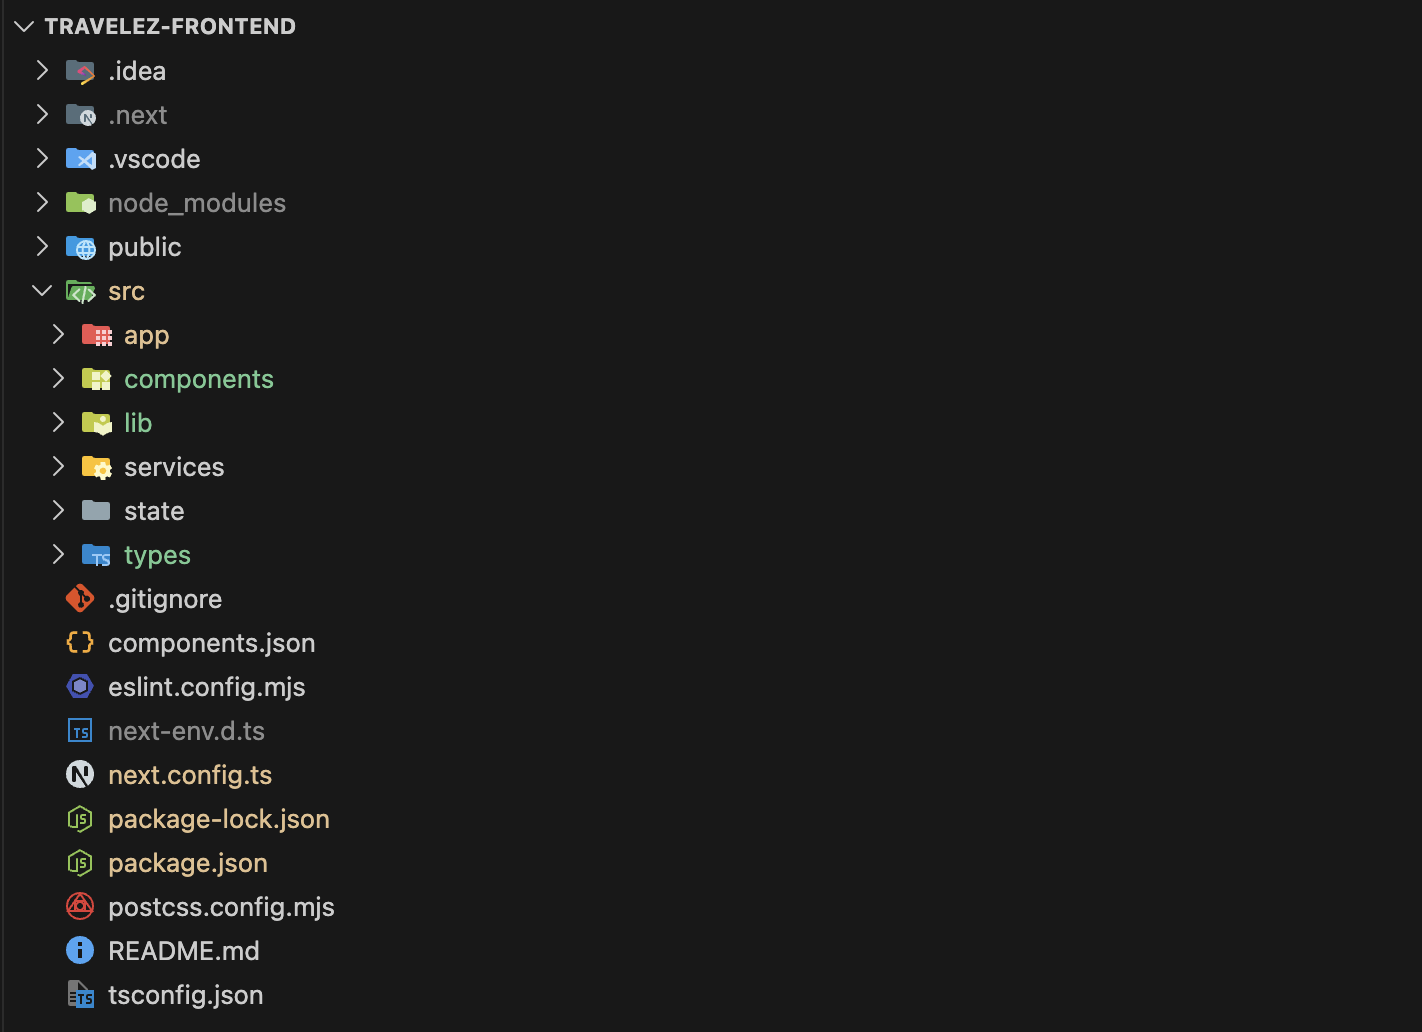
\includegraphics[width=1\textwidth]{Images/8. Implement/frontend-folder.png}
    \caption{Cấu trúc thư mục Frontend của TravelEZ}
    \label{fig:frontend-folder-structure}
\end{figure}

\subsubsection{Hướng dẫn chạy dự án}
Để thiết lập môi trường phát triển và chạy ứng dụng Frontend trên máy cục bộ, nhóm phát triển thực hiện theo quy trình sau:
\begin{enumerate}
    \item \textbf{Cài đặt thư viện:} \\
    Tại thư mục gốc của dự án, chạy lệnh sau để tải toàn bộ các gói phụ thuộc (dependencies) được khai báo trong file \texttt{package.json}:
    \begin{lstlisting}[language=bash, frame=single, basicstyle=\ttfamily]
npm install
    \end{lstlisting}

    \item \textbf{Khởi chạy môi trường phát triển:} \\
    Kích hoạt server phát triển của Next.js với tính năng Hot Reloading:
    \begin{lstlisting}[language=bash, frame=single, basicstyle=\ttfamily]
npm run dev
    \end{lstlisting}

    \item \textbf{Truy cập ứng dụng:} \\
    Sau khi server khởi động thành công, ứng dụng sẽ khả dụng tại địa chỉ trình duyệt: \texttt{http://localhost:3000}
\end{enumerate}
